\documentclass[handout]{beamer}
\usepackage{verbatim}
\usepackage{xcolor}
\usepackage{multirow}
\usepackage{amssymb}
\usepackage{tikz}
\usetikzlibrary{positioning,fit}
%\usepackage{enumitem}
\usetheme{Warsaw}
\setbeamertemplate{navigation symbols}{}
\newcommand{\blue}[1]{{\color{blue} #1}}
\newcommand{\red}[1]{{\color{red} #1}}
\newcommand{\grn}[1]{{\color{green} #1}}
\newcommand{\bluRed}[2]{{\color{blue} #1}{\color{red} #2}}
\newcommand{\qtns}[0]{\begin{center} Questions? \end{center}}
\newcommand{\nl}[1]{\vspace{#1 em}}
\newcommand{\cntrImg}[2]{\begin{center}\includegraphics[scale=#2]{#1}\end{center}}
\newcommand{\defn}[1]{{\bf #1}}
\let\emptyset\varnothing
\newcommand{\SampS}[0]{$\mathcal{S}$}

\title{Math 3070, Applied Statistics}

\begin{document}

\begin{frame}
    \begin{beamercolorbox}[rounded=true,wd=\textwidth,center]{title}
        \usebeamerfont{title}\inserttitle
    \end{beamercolorbox}
    \begin{center}
        Section 1\\
        \nl{0.5}
        September 23, 2019
    \end{center}
\end{frame}

\begin{frame}{Lecture Outline, 9/23}
    Section 4.2
    \begin{itemize}
        \item Cumulative Distribution Functions
        \item Expected Value and Variance of a Continuous Random Variable
    \end{itemize}
\end{frame}
\begin{frame}{Preface}
    Most definitions for continuous random variables change $\sum$ to $\int$ and usually work the same way.
\end{frame}
\begin{frame}{CDF of Continuous Random Variable}
    \begin{block}{}
        The \textbf{cumulative distribution function} (CDF), $F(x)$, of a continuous random variable $X$ is defined the same as in the discrete case:
        $$F(x) = P(X \leq x)$$
        If $X$ has pdf $f(x)$, then this becomes
        $$F(x) = \int_{-\infty}^x f(t)\ dt$$
    \end{block}
    \pause By the Fundamental Theorem of Calculus, $F'(x)=f(x)$, if $F'(x)$ exists at $x$.
    \vspace{-.5cm}
    \begin{center}
        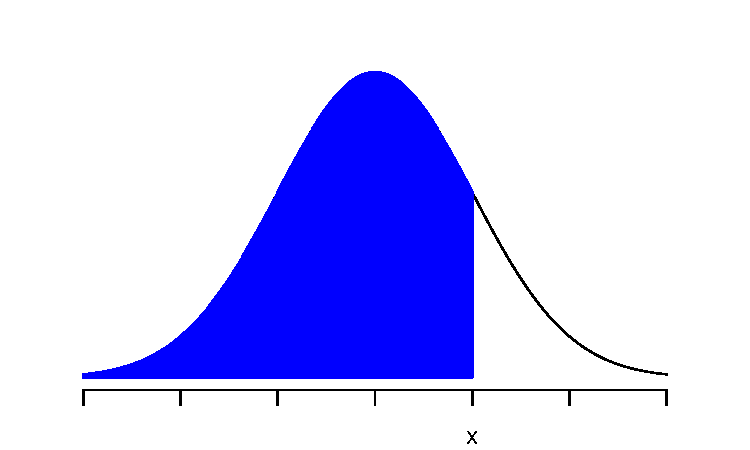
\includegraphics[scale=.4]{ch4_cdf_norm.pdf}
    \end{center}
\end{frame}
\begin{frame}{Example, CDF of $Unif(0,1)$}
    Compute the CDF of $X \sim unif(0,1)$.
    \\ \nl{0.5}
    \pause $$f(x)=\begin{cases} 1 & \text{if }0\leq x <1 \\
            0 & \text{otherwise}\end{cases} $$
    \pause
    When $x<0$,
    \pause $$P(X<x) = \int_{-\infty}^x f(x) dx = \int_{-\infty}^x 0 dx =0.$$
    When $0<x<1$,
    \pause $$P(X<x) = \int_{-\infty}^x f(x) dx = \int_{0}^x 1 dx =x.$$
    When $1<x$,
    \pause $$P(X<x) = \int_{-\infty}^x f(x) dx = \int_{0}^1 1 dx =1.$$
\end{frame}
\begin{frame}{Example, CDF of $Unif(0,1)$}
    Compute the CDF of $X \sim unif(0,1)$.
    \vfill
    $$F(x)=\begin{cases} 0, & x <0       \\
            x, & 0\leq x <1 \\
            1, & 1\leq x    \\
        \end{cases}$$
    \vfill
\end{frame}
\begin{frame}{Properties of CDFs}
    Useful for calculation:
    \begin{itemize}
        \item $P(X>a)=1-F(a)$
        \item $P(a\leq X \leq b)=F(b)-F(a)$
    \end{itemize}
    Useful for double-checking a function is a CDF:
    \begin{itemize}
        \item $\lim_{x\to -\infty}P(X<x) =0$
        \item $\lim_{x\to \infty}P(X<x) =1$
        \item CDFs of continuous random variables are continuous.
    \end{itemize}
\end{frame}
\begin{frame}{Percentiles and Median, Definition}
    \begin{block}{}
        Let $p$ be a number between 0 and 1. The $\mathbf{(100p)^{th}}$ \textbf{ percentile} of the distribution of a continuous random variable $X$ is denoted by $\eta(p)$ and defined by
        $$ p = F(\eta(p))= \int_{-\infty}^{\eta(p)} f(y)dy$$
    \end{block}
    Alternatively, $\eta(p) = F^{-1}(p)$ if $F(x)$ is invertible. If it's not we usually take the smallest $\eta(p)$ that suffices. Won't need to consider that in this class.
    \begin{block}{}
        The \textbf{median} $\tilde{u}$ of a continuous random variable $X$ is the $50^{th}$ percentile or the percentile with $p=0.5$.
    \end{block}
    This corresponds to the median of a data set. Roughly half of the observations will be below $\tilde{u}$.
\end{frame}
\begin{frame}{Example, Median}
    Calculate the median of a random varible with the following PDF:
    $$f(x)=\begin{cases} e^{-x+1} & \text{if }1\leq x \\
            0        & \text{otherwise}\end{cases} $$
    \pause When $x<1$,
    \pause $$ P(X<x) = \int_{-\infty}^x f(x) dx = 0$$
    \pause When $x\geq 1$,
    \pause
    \begin{align*} P(X<x) & = \int_{-\infty}^x f(x) dx = \int_{1}^x e^{-s+1} ds \\
               & = -e^{-s+1}\bigg|_{s=1}^x = 1 - e^{-x+1}
    \end{align*}
\end{frame}
\begin{frame}{Example, Median}
    Calculate the median of a random varible with the following PDF:
    $$F(x)=\begin{cases} 1- e^{-x+1}, & \text{if }1\leq x \\
            0,           & x<1
        \end{cases}$$
    \pause $F(x) = 0.5$ when $x\geq 1$. Need to invert the function in that region.
    \pause
    \begin{align*}
        0.5            & = 1 - e^{-\tilde{u}+1} \\
        0.5            & = e^{-\tilde{u}+1}     \\
        \ln{(0.5)}     & = -\tilde{u}+1         \\
        1 - \ln{(0.5)} & = \tilde{u}            \\
        \tilde{u}      & \approx 1.69315
    \end{align*}
    \vfill
\end{frame}
\begin{frame}{Summary, Cumulative Density Function}
    \begin{itemize}
        \item CDF: $F(x) = P(X<x) = \int_{-\infty}^x f(t) dt$
        \item $F'(x) = f(x)$ when $F'(x)$ exists.
        \item $P(X>a)=1-F(a)$
        \item $P(a\leq X \leq b)=F(b)-F(a)$
        \item $\lim_{x\to -\infty}P(X<x) =0$
        \item $\lim_{x\to \infty}P(X<x) =1$
        \item CDFs of continuous random variables are continuous.
        \item $100p^{th}$ percentile $\eta(p)$: $p=F(\eta(p))$
        \item median $\tilde{u}$, $p=0.5$ percentile
    \end{itemize}
\end{frame}
\begin{frame}{Expected Value, Definition}
    \begin{block}{}
        The \textbf{expected value} or \textbf{mean} of a continuous random variable $X$ with PDF $f(x)$ is
        $$ \mu_X = E(X) = \int_{-\infty}^\infty x \cdot f(x) dx.$$
        If $h(x)$ is a function then
        $$ E[h(X)] = \int_{-\infty}^\infty h(x) \cdot f(x) dx.$$
    \end{block}
    Mean has the same interpretation as the discrete case or from data, a measure of center or location. And, it is also linear,
    $$ E[g(X) + ah(X) + b] = E[g(X)]+ a E[h(x)] + b.$$
    Why? Integrals are linear.
\end{frame}
\begin{frame}{Variance, Definition}
    \begin{block}{}
        The \textbf{variance} of a continuous random variable $X$ with PDF $f(x)$ and $E[X] = \mu$ is
        $$ \sigma^2_X = V(X) = \int_{-\infty}^\infty (x-\mu)^2 \cdot f(x) dx=E[(X-\mu)^2].$$
        The \textbf{standard deviation} (SD) of $X$ is $\sigma_x = \sqrt{V(X)}$.
    \end{block}
    Same interpretation, average spread. Shorcut formula and linear transforms work the same too.
    $$ V(X) =  E[X^2] - E[X]^2$$
    $$ V(aX +b) = a^2V(X) $$
    \vfill
\end{frame}
\begin{frame}{Variance, Derivations for Shortcut Formula and Linear Transforms}
    Shortcut Formula:
    \begin{align*}
        V(X) & = \int_{-\infty}^\infty (x-\mu)^2 \cdot f(x) dx \\
        &= \int_{-\infty}^\infty (x)^2 \cdot f(x) dx -2 \mu \int_{-\infty}^\infty x \cdot f(x) dx + \mu^2 \int_{-\infty}^\infty  f(x) dx\\
        &= E[X^2] - \mu^2 = E[X^2] - E[X]^2
    \end{align*}
    Linear Transforms:
    Note: $E[aX + b] = aE[X] + b = a\mu +b$
    \begin{align*}
        V(aX + b) & = \int_{-\infty}^\infty [ax+b -(a\mu+b)]^2 \cdot f(x) dx \\
        &= \int_{-\infty}^\infty a^2 [x-\mu]^2 \cdot f(x) dx \\
        &= a^2 V(X)\\
    \end{align*}
\end{frame}
\begin{frame}{Example, Mean and Variance of the a Uniform RV}
    Compute the mean and variance of $X\sim unif(a,b)$.
    \pause
    $$f(x)=\begin{cases} \frac{1}{b-a}, & a \leq x <b      \\
        0, & \text{otherwise} \\
    \end{cases}$$
    \pause guess.
    \pause
    \begin{align*}
         E[X] &= \int_{-\infty}^\infty xf(x) dx = \int_{a}^b \frac{x}{b-a} dx\\
         & = \frac{x^2}{2(b-a)} \bigg|_a^b = \frac{b^2 - a^2}{2(b-a)}\\
         \pause & =\frac{(b-a)(b+a)}{2(b-a)} = \frac{b+a}{2}
    \end{align*}
    \vfill
\end{frame}
\begin{frame}{Example, Mean and Variance of the a Uniform RV}
    Compute the mean and variance of $X\sim unif(a,b)$.
    \pause
    $$f(x)=\begin{cases} \frac{1}{b-a}, & a \leq x <b      \\
        0, & \text{otherwise} \\
    \end{cases}$$
    \begin{align*}
         V(X) &= E[X^2] - E[X]^2\\
         & = \int_a^b \frac{x^2}{b-a} dx - \bigg( \frac{b+a}{2} \bigg)^2 = \frac{1}{b-a} \frac{x^3}{3}\bigg|_{x=a}^b - \bigg( \frac{b+a}{2} \bigg)^2\\
         & = \frac{b^3 - a^3}{3(b-a)}  - \bigg( \frac{b+a}{2} \bigg)^2 = \frac{(b-a)(a^2+ab+b^2)}{3(b-a)}  - \bigg( \frac{b+a}{2} \bigg)^2\\
         & = \frac{(a^2+ab+b^2)}{3}  - \frac{b^2+2ba + a^2}{4} \\
         &= \frac{(4a^2+4ab+4b^2)}{12}  - \frac{3b^2+6ba + 3a^2}{12}\\
         & = \frac{a^2 - 2 ab + b^2}{12} = \frac{(b-a)^2}{12}
    \end{align*}
    \vfill
\end{frame}
\begin{frame}{Example, Mean and Variance of the a Uniform RV}
    Compute the mean and variance of $X\sim unif(a,b)$.
    $$ E[X] = \frac{b+a}{2} $$
    $$ V(X) = \frac{(b-a)^2}{12}$$
    Takeaway:
    \begin{itemize}
        \item The mean is the average of the end points.
        \item The variance is explictly related to the distance between the endpoints $b-a$.
    \end{itemize}
    \vfill
\end{frame}
\begin{frame}{Example, Modeling with a Uniform RV}
    A random number generator produces values that follow uniform random variable. Researchers take find a sample mean of 5 and a sample standard deviation of $\sqrt{12}$. Determine the minimum and maximum values assuming that the sample mean and variance are the true mean and standard deviation. \\ \nl{0.5}
    \pause Using what was found in the previous problem,
    $$ \frac{b+a}{2} = 5 \text{ and } \frac{b-a}{\sqrt{12}} = \sqrt{12}$$
    or
    $$ b+a = 10 \text{ and } b-a = 12$$
    \pause Using linear algebra,
    $$ b =11 \text{ and } a = -1 .$$
    Maximum value $=11$ and minimum value $= -1$.
    \vfill
\end{frame}
\begin{frame}{Example, Modeling with a Uniform RV}
    A random number generator produces values that follow uniform random variable. Researchers take find a sample mean of 5 and a sample standard deviation of $\sqrt{12}$. Determine the minimum and maximum values assuming that the sample mean and variance are the true mean and standard deviation. \\ \nl{1}
    Closing note, $P(X=b)=P(X=a)=0$ or it is impossible to observe the endpoints of a uniform random variable. Maximum and minimum values of the data set may not work as well as the sample mean and variance.
    \vfill
\end{frame}
\begin{frame}{Summary, Expected Value and Variance}
    \begin{itemize}
        \item $\mu_X = E(X) = \int_{-\infty}^\infty x \cdot f(x) dx$
        \item $E[h(X)] = \int_{-\infty}^\infty h(x) \cdot f(x) dx$
        \item $E[g(X) + ah(X) + b] = E[g(X)]+ a E[h(x)] + b$ 
        \item $\sigma^2_X = V(X) = \int_{-\infty}^\infty (x-\mu)^2 \cdot f(x) dx=E[(X-\mu)^2]$
        \item $ V(X) =  E[X^2] - E[X]^2$
        \item $ V(aX +b) = a^2V(X) $
        \item If $X\sim unif(a,b)$
        $$E[X] = \frac{b+a}{2} \hskip 1em V(X) = \frac{(b-a)^2}{12}$$
    \end{itemize}
\end{frame}
\end{document}